\documentclass[twocolumn,english]{IEEEtran}
\usepackage[T1]{fontenc}
\usepackage{babel}
\usepackage{amsthm}
\usepackage{amsmath}
\usepackage{graphicx}
\usepackage[unicode=true,
 bookmarks=true,bookmarksnumbered=true,bookmarksopen=true,bookmarksopenlevel=1,
 breaklinks=false,pdfborder={0 0 0},backref=false,colorlinks=false]
 {hyperref}
\usepackage{bm}
\usepackage{amsmath}
\usepackage{amssymb}
\usepackage{natbib}
\usepackage{array}
\usepackage{calc}
\newcolumntype{W}{>{\centering\arraybackslash}m{25mm}}
\newcolumntype{L}{>{\centering\arraybackslash}m{15mm}}


\hypersetup{
 pdftitle=  {Lab 6: Electric Power},
 pdfauthor= {Zack Garza},
 pdfpagelayout=OneColumn, pdfnewwindow=true, pdfstartview=XYZ, plainpages=false}

\makeatletter


%%%%%%%%%%%%%%%%%%%%%%%%%%%%%% Textclass specific LaTeX commands.
 % protect \markboth against an old bug reintroduced in babel >= 3.8g
 \let\oldforeign@language\foreign@language
 \DeclareRobustCommand{\foreign@language}[1]{%
   \lowercase{\oldforeign@language{#1}}}
\theoremstyle{plain}
\newtheorem{thm}{\protect\theoremname}
\theoremstyle{plain}
\newtheorem{lem}[thm]{\protect\lemmaname}

%%%%%%%%%%%%%%%%%%%%%%%%%%%%%% User specified LaTeX commands.
% for subfigures/subtables
\ifCLASSOPTIONcompsoc
\usepackage[caption=false,font=normalsize,labelfont=sf,textfont=sf]{subfig}
\else
\usepackage[caption=false,font=footnotesize]{subfig}
\fi

\makeatother
\providecommand{\lemmaname}{Lemma}
\providecommand{\theoremname}{Theorem}
\setcounter{topnumber}{2}
\setcounter{bottomnumber}{2}
\setcounter{totalnumber}{4}
\renewcommand{\topfraction}{0.85}
\renewcommand{\bottomfraction}{0.85}
\renewcommand{\textfraction}{0.15}
\renewcommand{\floatpagefraction}{0.7}
\usepackage{float}
\begin{document}

\title{Lab Name}


\author{Zack Garza}


\IEEEspecialpapernotice
{Physics 210L \\
Effective Date of Report: \today}


\markboth{Electric Power}{Zack Garza}
\maketitle
\begin{abstract}
\IEEEPARstart{T}{his} is a placeholder
\end{abstract}
\tableofcontents

\section{Theory}
\begin{figure}[h!]
  \begin{centering}
  \begin{center}
  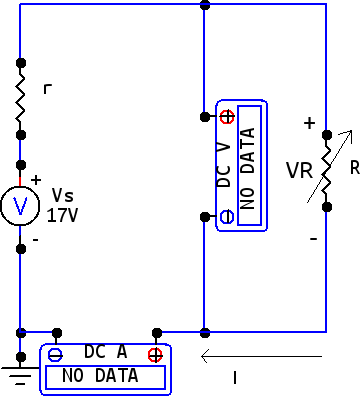
\includegraphics[width=\linewidth]{./circuit.png}
  \caption{Diagram of circuit used in this experiment. $R$ represents a variable load resistance, while $r$ simulates the internal resistance of the power supply. $I$ is the uniform current that flows through all three components of the circuit.}
  \label{fig:circuit_diagram}
  \end{center}
  \par\end{centering}
  \end{figure}

\textbf{Kirchoff's Voltage Law} states that the sum of the potential differences in a closed loop is equal to zero, such that
\begin{equation*}
 \sum V_{\text{Loop}} = 0.
\end{equation*}

For the circuit shown, the potential difference $V_R$ across the load resistor can be found using this equation. Summing the voltages and rewriting them using $V=iR$ (according to Ohm's Law) yields
\begin{align}\label{eq:part1}
 \epsilon - V_{r} - V_R &= 0 	\Rightarrow \notag \\
 V_R &= \epsilon - V_r 		\Rightarrow \notag \\
 V_R &= \epsilon - ir
\end{align}
where the current $i$ is identical throughout the circuit, as its elements are wired in series, and $r$ is the power supply's internal voltage.

The power released by the resistor $R$ can also be expressed in terms of the known quantities $\epsilon, r$, and $R$. From the power equation, it is known that $P=iV$. Because the current $i$ is uniform everywhere, it can be related to the source voltage and the equivalent resistance of the entire circuit. Taking the source voltage to as $\epsilon$ and the equivalent resistance as $r+R$ and substituting it into the power equation yields
\begin{align}\label{eq:part2}
 P = iV, V = iR \Rightarrow P = \frac{i^2}{R} 	\Rightarrow \notag 	\\
 P_R = \left(\frac{\epsilon}{r+R}\right)^2 R 	\Rightarrow \notag	\\
 P_R = \epsilon^2 \frac{R}{(r+R)^2}.
\end{align}

Calculating the point at which maximum power transfer occurs requires taking the derivative of Equation~\ref{eq:part2} with respect to the load resistance. This results in
\begin{align*}
 \frac{\partial P}{\partial R} = \epsilon^2 \left(\frac{(r+R^2)-2R(R+r)}{(R+r)^4}\right).
\end{align*}

Maximizing the power transferred to the load resistor requires setting this derivative equal to zero, which occurs when.
\begin{align*}
 r+R^2 = 2R(R+r).
\end{align*}

Solving this expression for $R$ then forces the following condition to be true in order to maximize the power delivered to the load resistor $R$:
\begin{align}
 R=r.
\end{align}

\section{Methodology}
\begin{enumerate}
 \item The circuit was constructed as shown in Figure~\ref{fig:circuit_diagram}, where $r$ was a known resistor and $R$ was a variable resistor box.
 \item Digital voltmeters and ammeters were wired to measure $V_R$ and $i$.
 \item The power supply was set to 17.00 V, and its actual terminal voltage was measured.
 \item The known resistor $r$ was measured with an ohmmeter.
 \item The resistance of the variable load was incremented, and at each point data was taken for the voltage and current through $R$.
 \item Extra data points were taken at resistances approaching that of the known resistor.
\end{enumerate}

\noindent \hrulefill

\section{Data}
\begin{align*}
 r &= .549 \text{ k}\Omega \\
 \epsilon_{\text{Meas}} &= 17.02 \text{ V}
\end{align*}

  \subsection{\textbf{Linear Fit of $V_R$ vs. $i$}}
  \begin{align*}
   \text{Internal Resistance $r$} 		&=\text{\underline{$(571 \pm 2)\Omega$}}	\\
   \text{Source EMF }\mu_{\text{Theory}}	&=\text{\underline{$(16.99 \pm .04)$V}}
  \end{align*}

  \begin{align*}
   \text{\% Difference in }\epsilon 	&=\text{\underline{0.2\%}}	\\
   \text{\% Difference in }r		&=\text{\underline{3.9\%}}
  \end{align*}

  \subsection{\textbf{Comparison of $R_{\text{Calc}}$ and Resistance Box Values}}
  Filler text.

  \subsection{\textbf{Polynomial Fit of $P_R$ vs. $R_{\text{Calc}}$}}
  \begin{align*}
   r 				&= \text{\underline{$(573.2 \pm 0.7)\Omega$}}	\\
   \text{\% Difference} 	&= \text{\underline{0.38\%}}
  \end{align*}

\section{Analysis}
\begin{enumerate}
 \item \textit{How can you determine the value for $R_{\text{Calculated}}$ that gives $P_{\text{R-Max}}$?}
 \item \textit{What are the possible discrepancies between the values of $r$ obtained from the two function fits?}
\end{enumerate}


\appendices{}

%\bibliographystyle{plain}
%\bibliography{physbib}

\end{document}